%MRC5December2012 -- Added a bit about  the corporate partner context
%Context
\chapterimage{ChapterImages/context}
\chapter{Context}\label{sec-context} %Label for cross-referencing

% %%%%%%%%%%%%
% \begin{remark} \color{blue}
% {\Large What need are you addressing for your users and your company?}

% \noindent The Context provides background and motivation for your project. It is an enlarged version of the brief context in your Executive Summary.  
% \begin{itemize} %\tightlist
% \item Who came to you with a proposed project area? Who is the corporate partner and what is their context?
% \item What background or context set the stage for your Needfinding and Benchmarking, activities?
% \end{itemize}
% Suggested length: Up to half a page to a page each for the Need Statement and Problem Statement (plus figures, if any). Another page or two for the design team.
% \normalcolor \end{remark}
% %%%%%%%%%%%%

\section{Design Challenge}
\label{sec:challenge}

The technology around home and car has changed dramatically in the last decade with autonomous driving, voice control and the Internet of Things (IoT) being the most prominent of these developments. For this project, we were given the following challenge: With the smart home promising a future of convenience and intelligence at home, what could the future hold for Audi?

\todo{picture for business canvas looks cutoff at top and has icons in lower left}

\begin{figure}[ht]
	\centering
	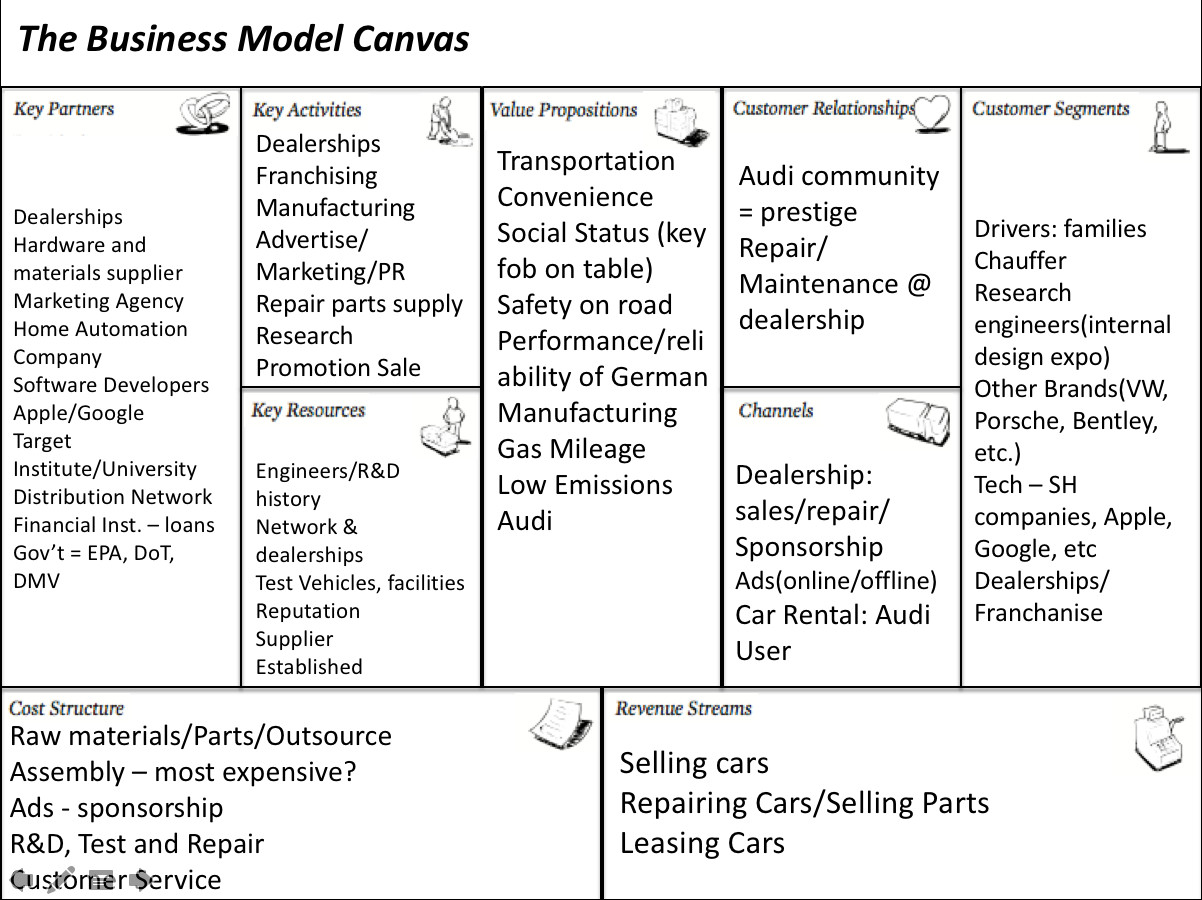
\includegraphics[width=5.9in]{Figures/ChapterContext/canvas.png}
	\caption{The business canvas that identifies the business model of Audi and related stakeholders}
	\label{fig:canvas}
\end{figure}

\section{Problem Statement}

The focus of our work is to create an integration of the Audi brand into the smart home. Most desirable would be a physical representation of Audi in the home since that would expand Audi's perceived value beyond that of a car maker. This brings up the question that we currently work on:

\begin{center}
\textbf{How can Audi play a meaningful role in the emerging smart home market\\or integrate itself with the promises of smart home technology?}
\end{center}

\section{Corporate Partner: Audi}
\label{subsec:audi}

The automobile manufacturer Audi is the corporate partner for this project. As a major producer of luxury cars, Audi has always been at the forefront of automobile technology -  both in driving experience and comfort features of the car. The latest technological innovations are usually implemented into the most expensive series first. Subsequently, they make their way down the line-up, appearing in more affordable models every year. Audi produces a wide range of vehicles from sedans to sport utility vehicles ~\cite{Audi2014Winter}.

Fig. \ref{fig:canvas} describes the team's understanding of the Audi brand and the Volkswagen corporation. As a traditional car manufacturer, Audi's revenue mainly comes from selling cars, its cost consists of raw materials, machining, assembly, advertisement, Research and Design (R\&D), test and customer service. Audi's key resources are threefold: first is the work of engineers and its R\&D achievements, second is its distribution network and dealerships, and third is its brand and reputation. The key value proposition of Audi is convenience and fun of driving, being considered a social status symbol, delivering great performance, as well as providing the reliability of German engineering and its experience with advanced technology.
% \begin{remark} \color{blue}
% \textit{I didn't understand this sentence and hope I could capture its meaning with the following paragraph (I would argue that prestige is already captured in "social status symbol" of the preceding paragraph):}
% Audi has a emphasis on custom relationship, because Audi community has a closely emotional bond to this brand, and an important part of the luxury brand is the prestige.
% \end{remark}
Audi maintains good relationships with customers who develop an emotional bond to it, making the relationship mutually beneficial.

%If possible, try to make this display on a whole page


The Electronics Research Laboratory (ERL) is the main contact point between the design team and Audi. It is is the direct link of Audi and other Volkswagen Group brands to Silicon Valley. Engineers here are encouraged to invent and experiment with innovative technological solutions and features that explore the opportunity space for future car generations. At the same time, the location benefits vastly of the proximity to the main drivers of the IT industry and elite educational institutions. Relevant research areas include human machine interface systems, driver assist systems, and infotainment applications and platforms ~\cite{Audi2012December}.

\begin{center}
% * <djmoore3@stanford.edu> 2015-12-10T16:37:20.003Z:
%
% > \begin{center}
% > 
\includegraphics{Figures/AUDI}
% > \vfill
% > 
\includegraphics{Figures/ERL}
% > \end{center}
%
% Can these graphics be better laid out?
%
% ^.


\includegraphics{Figures/Logos/AUDI}

% \vspace{1cm}


\includegraphics{Figures/Logos/ERL}

\end{center}

\clearpage

\subsection{Corporate Liaisons}

\vspace{1em}
\noindent 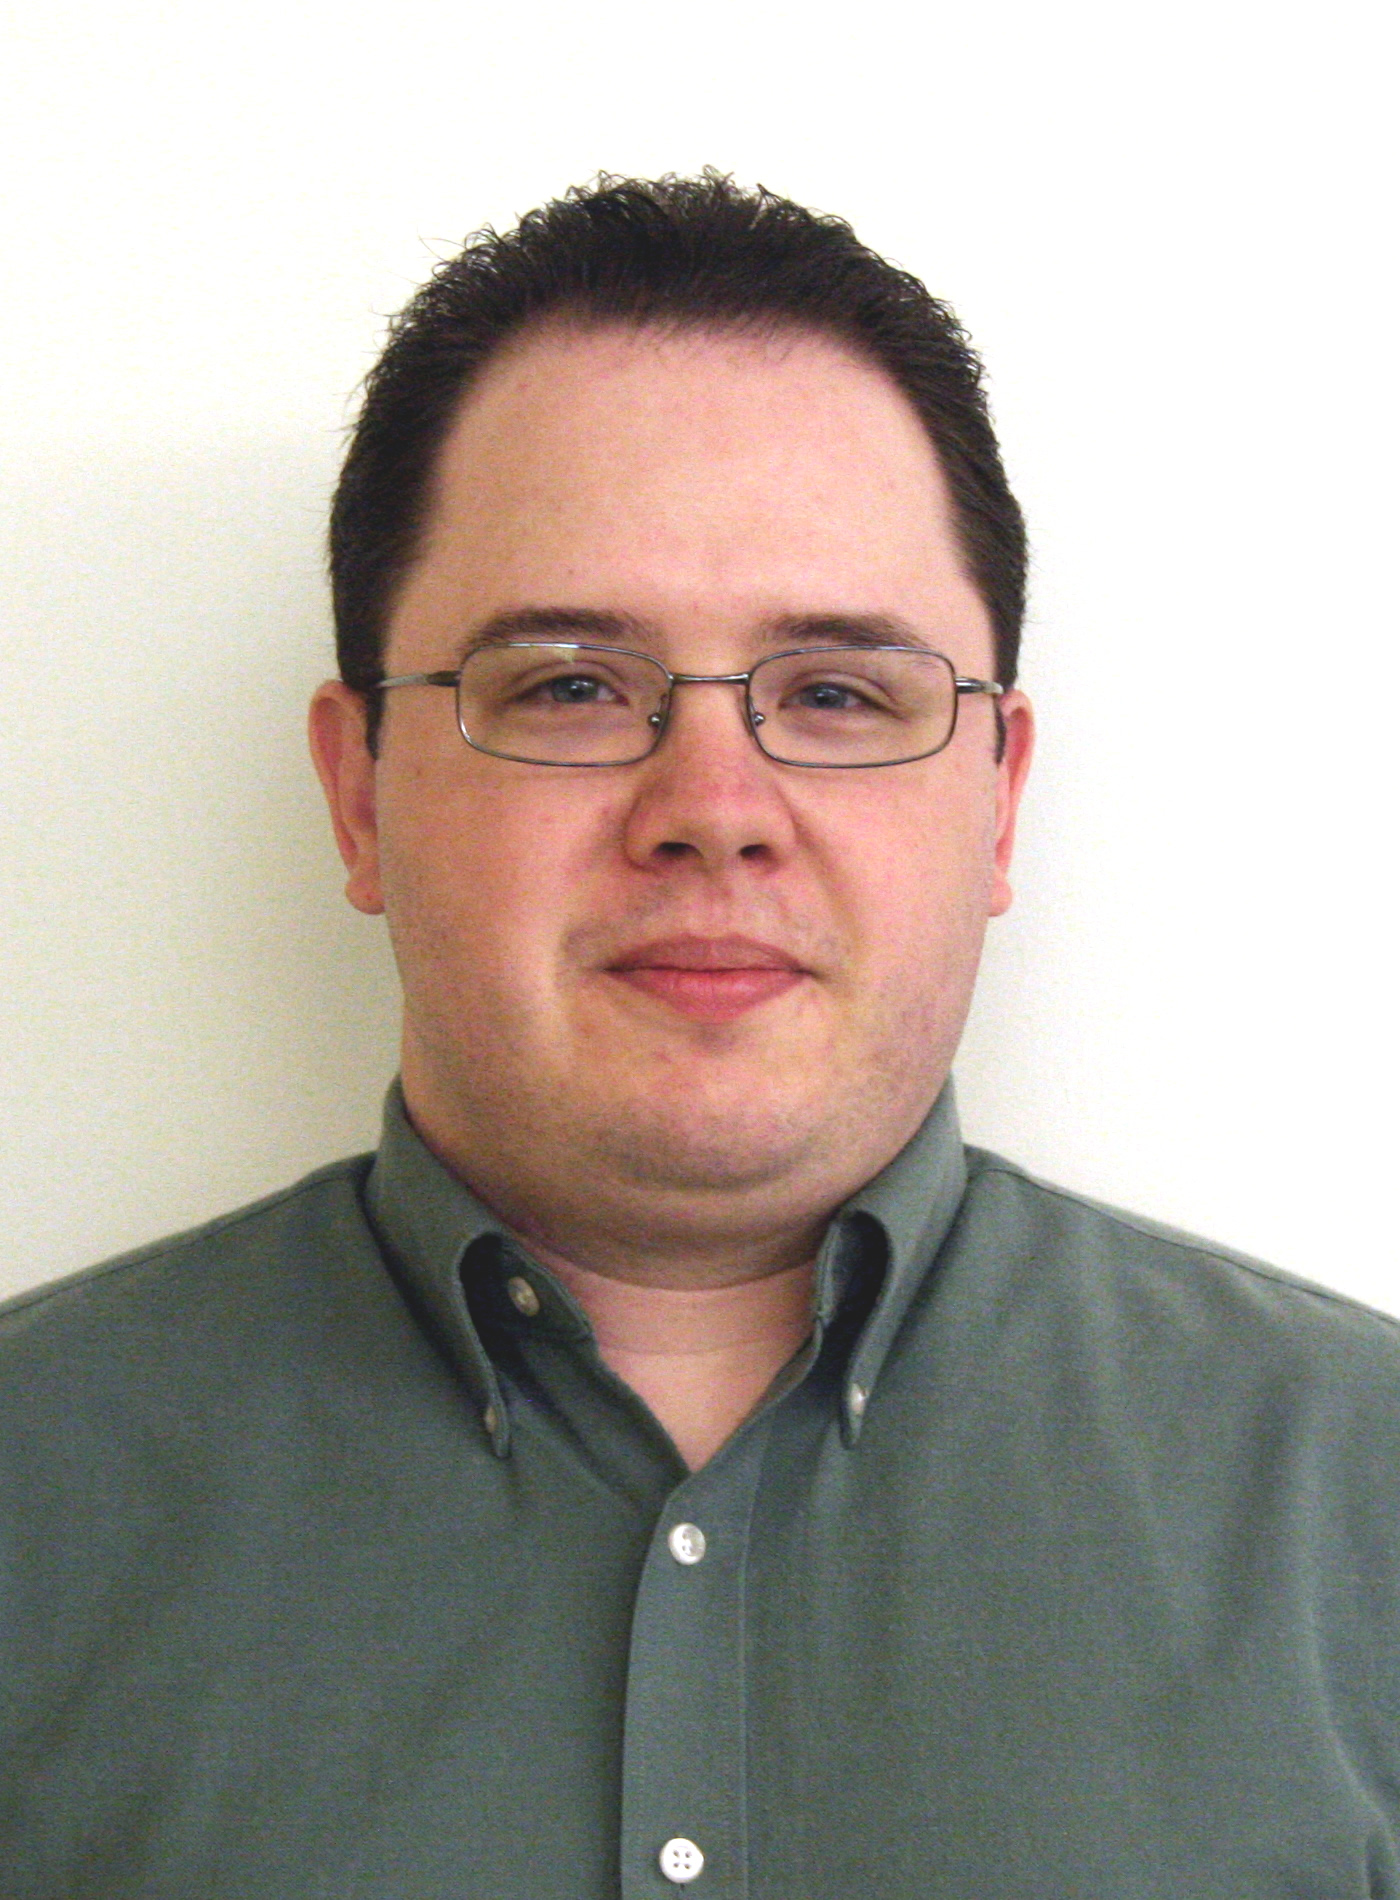
\includegraphics[width=35mm]{Figures/People/Nate}
\hspace{1em}\parbox[b]{0.6\textwidth}{\textbf{Nathaniel Coser}\\
Volkswagen-Electronics Research Laboratory\\
Contact: Nathaniel.Coser@vw.com\\
}
\vspace{2em}

\noindent 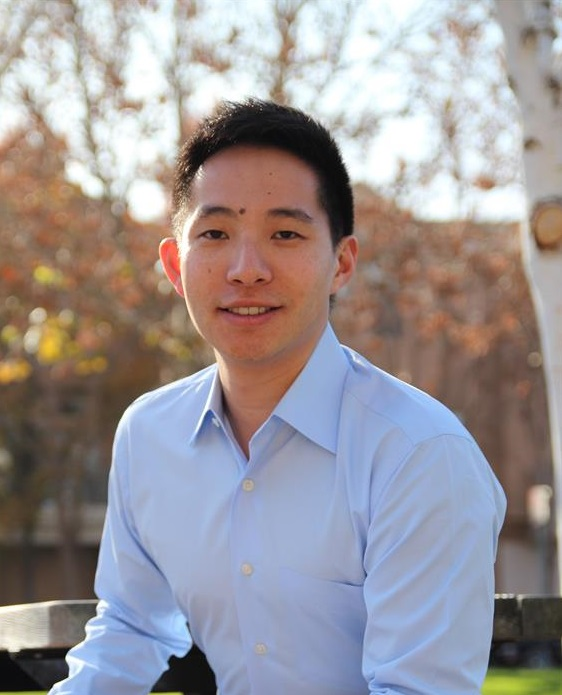
\includegraphics[width=35mm]{Figures/People/andrew}
\hspace{1em}\parbox[b]{0.6\textwidth}{\textbf{Andrew Chang}\\
Volkswagen-Electronics Research Laboratory\\
Contact: Andrew.Chang@vw.com\\
}
\vspace{2em}

\noindent 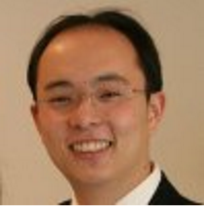
\includegraphics[width=35mm]{Figures/People/Henry}
\hspace{1em}\parbox[b]{0.6\textwidth}{\textbf{Henry Chen}\\
Volkswagen-Electronics Research Laboratory \\
Contact: Henry.Chen@vw.com\\
}

\clearpage

\section{The Design Team}
\label{sec:team}

The design team was assembled from individuals with a diversity of thinking preferences, interests and backgrounds. There is some evidence that such diversity enhances team creativity \cite{Wilde97, Wilde07} , even if it creates additional challenges for team management.

\subsection{Students}

% Example table. It gets a caption and reference label.
% The tabular formatting is a bit painful...  An alternative is to use Word
% and insert the PDF printout as for a figure. There are also Word-to-Latex converters.
%
%Nov2013 -- I decided to comment this out because corporate partners don't care about this. -MRC
%
%\begin{table}
%  \begin{tabular}{| p{14mm} | p{20mm} | p{20mm} | p{22mm} | p{20mm} | p{12mm} |} 
%  \hline
%Score & Extroverted-Introverted (E-I) & Intuition-Sensing (N-S) & Feeling-Thinking (F-T) & Perception-Judging (P-J) & Overall \\
%People & & & & &\\
%\hline
%Larry & +6 & +6 & -6 & +12 & ENTP \\
%Mark & -18 & +30 & -30 & +18 & INTP \\
%George & +6 & +18 & -18 & +6 & ENTP \\
%\hline
%\end{tabular}
%\caption{Team preferences scores using the method of Wilde \cite{Wilde07}. (These data are not real.)}
%	\label{wildeprefs}  %Tag for referring to table
%\end{table}

%\begin{framed}
%\noindent \includegraphics[width=40mm]{Figures/Ch2/LarryLeifer.jpg}
% \parbox[b]{0.6\textwidth}{Larry Leifer\\
% Status: Professor, Mechanical Engineering\\
% Contact: leifer@cdr.stanford.edu\\
% Skills: deisgn, mechatronics, welding, prototyping\\
% Computing: Solid Works, Matlab, basic C programming, Forth\\
% }
% %Note, the blank lines matter - they cause the start of a paragraph in the box.

% Born in Santa Barbara I remain a surfer at heart.
% My research is focused on instrumenting, understanding, supporting, and improving design practice through the development of design theory. BS in in Engineering Science, MS in Product Design, PhD in Biomedical Engineering, all from Stanford.
% Founder of the  Center for Design Research and one of the founding faculty members of the Hasso Plattner Design Institute
% at Stanford (aka the d.school).

% Favorite activities include surfing, hunting and wayfaring, and frequent trips to Lucerne, Switzerland.
%\end{framed}

%\begin{framed}
\vspace{0.5em}
\noindent 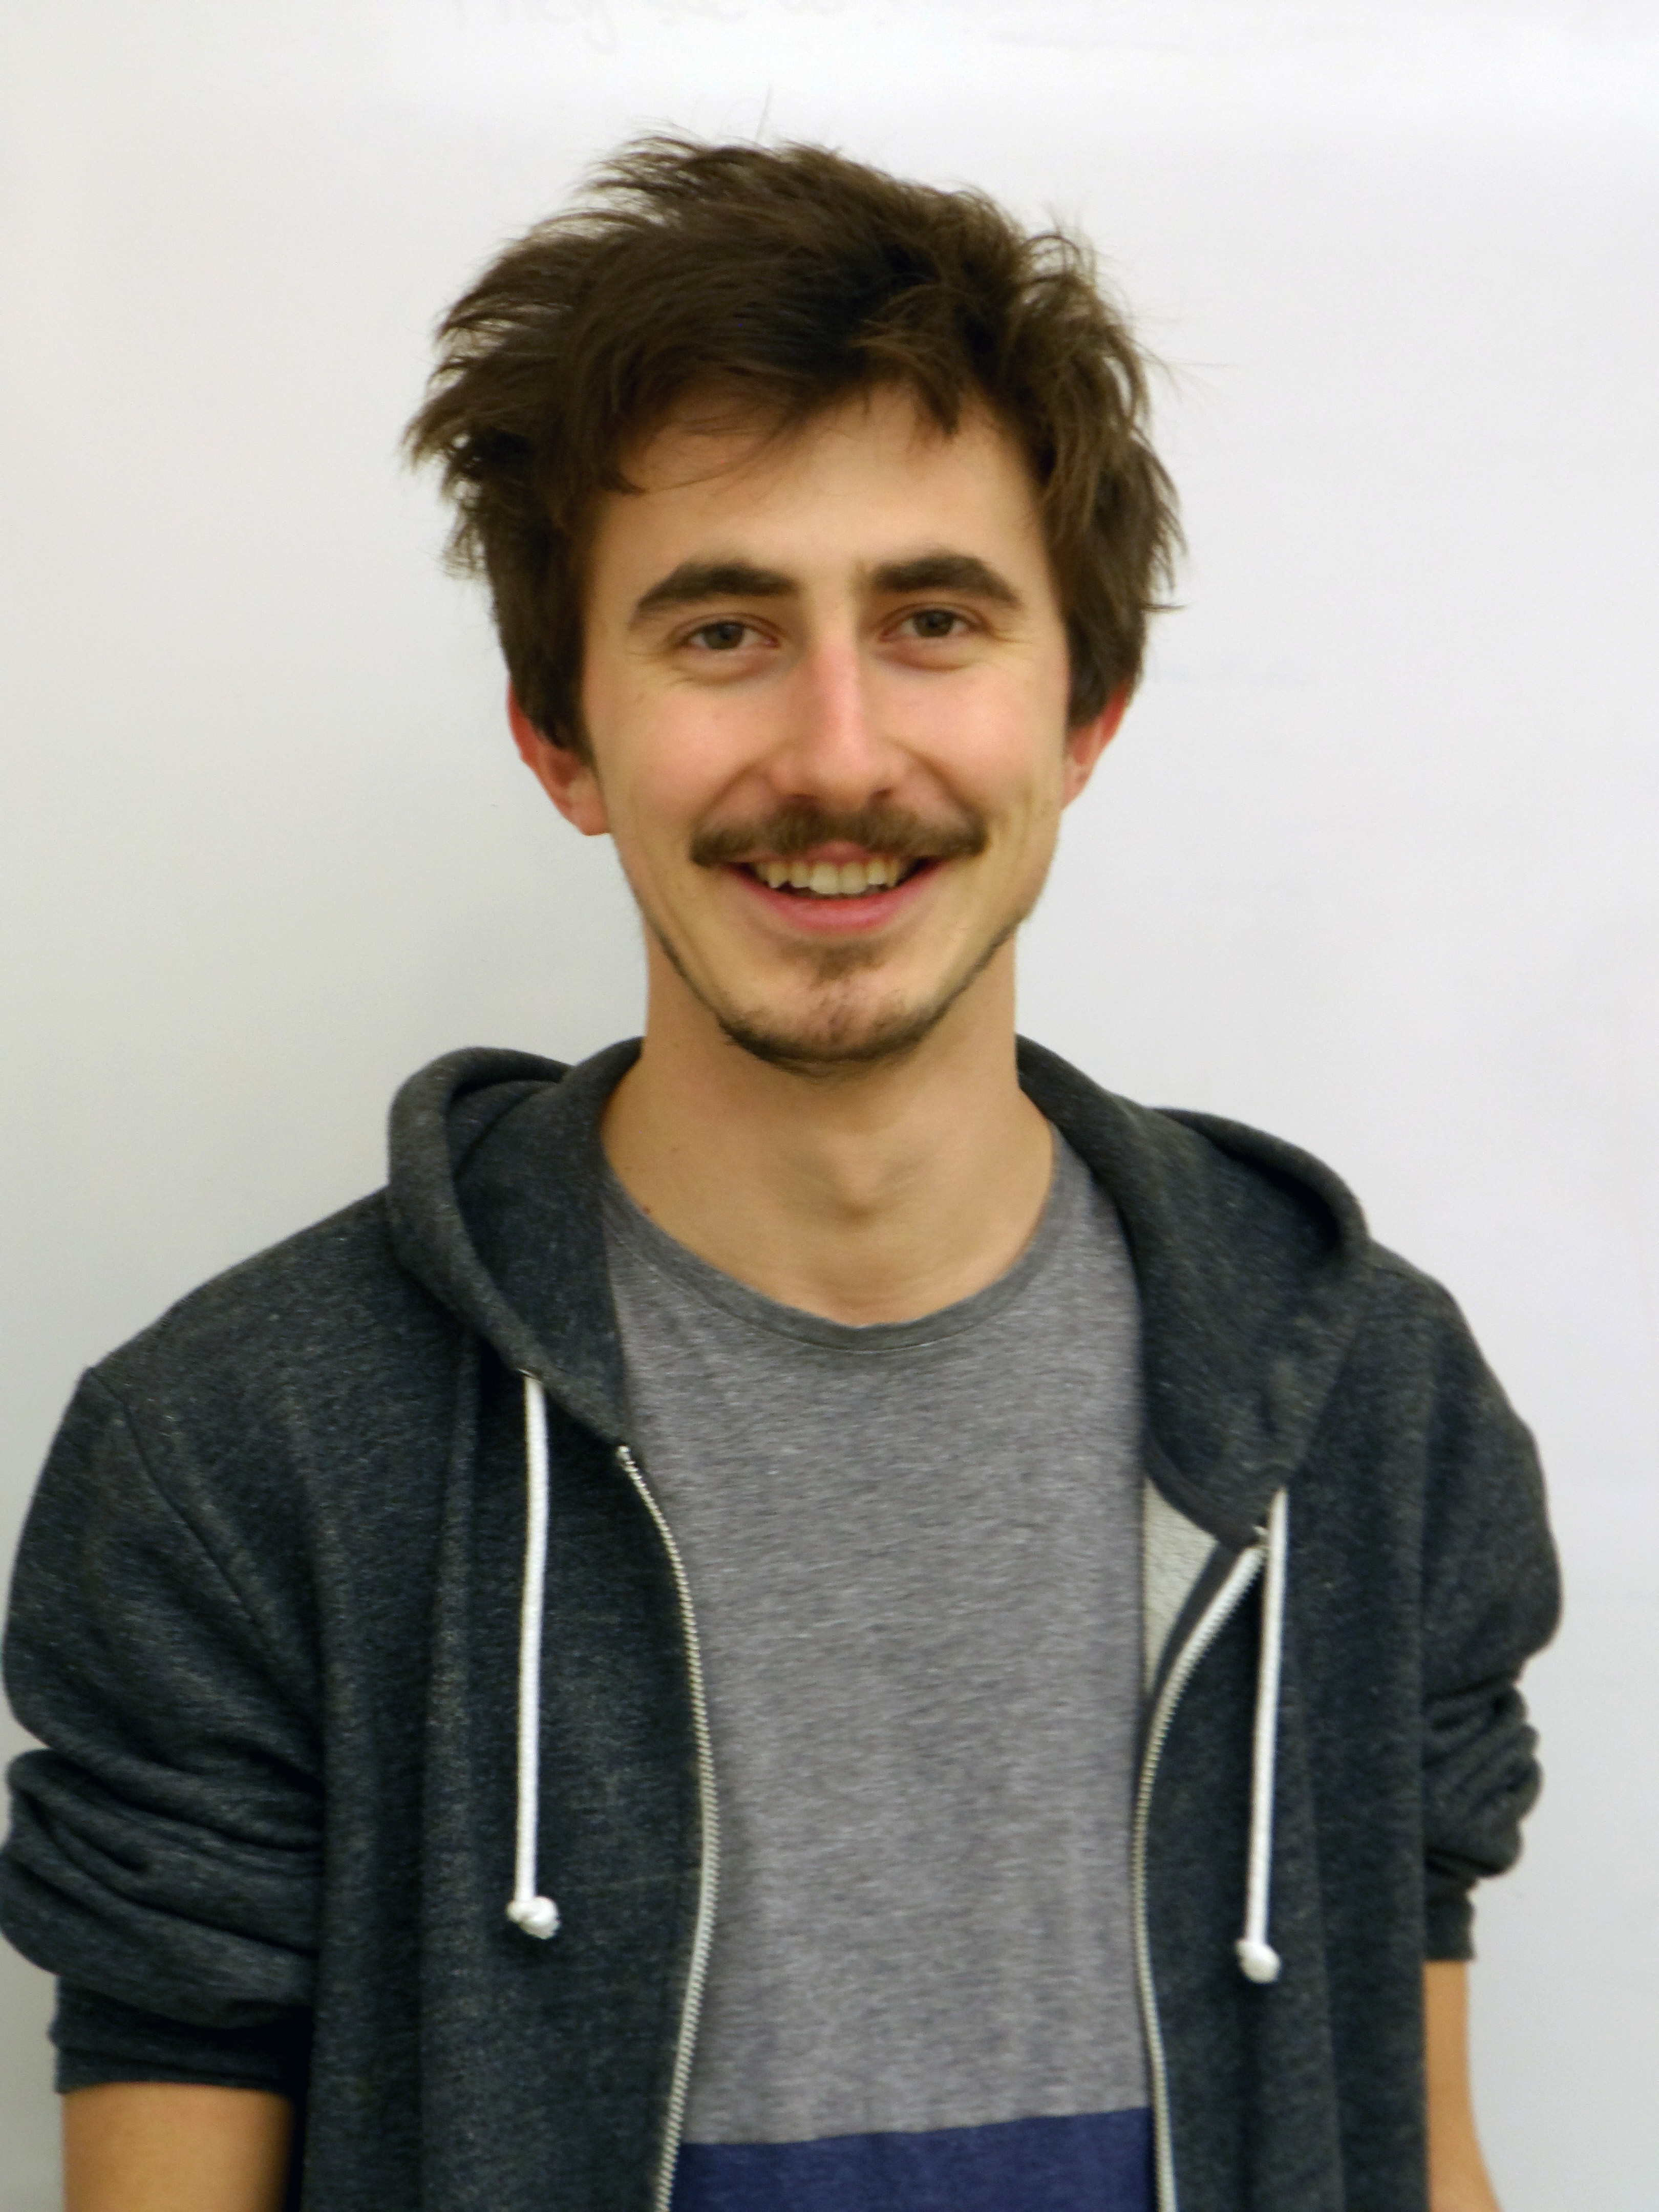
\includegraphics[width=35mm]{Figures/People/martin}
\hspace{0.5em}\parbox[b]{0.6\textwidth}{\textbf{Martin Fritzsche}\\
Hasso Plattner Institute\\
Status: IT-Systems Engineering Master's degree student\\
Contact: martin.fritzsche@student.hpi.de\\
Skills: Software Engineering, Human Computer Interaction, C++\\
}

I was born 1989 in the medium sized town Jena in the center of Germany. After finishing school there and spending a year in Dresden working in a hospital for civil service I started my studies at the Hasso Plattner Institute (HPI). In 2012, in between Bachelor and Master at HPI, I collected valuable working experience as full-time employee at Citrix Online Germany. In my masters studies I focused on human computer interaction, working on prototyping research and combining virtual reality with real life by taking control of the users muscles. Before starting the ME310 course this fall I spent one year at Universidad Politécnica de Madrid in Spain.

Besides virtual reality research and low level development I like hands-on experiences and interdisciplinary work. That is why I am happy to dive into the design thinking process and work on our real life project at ME310.
%\end{framed}

\vspace{2em}
\noindent 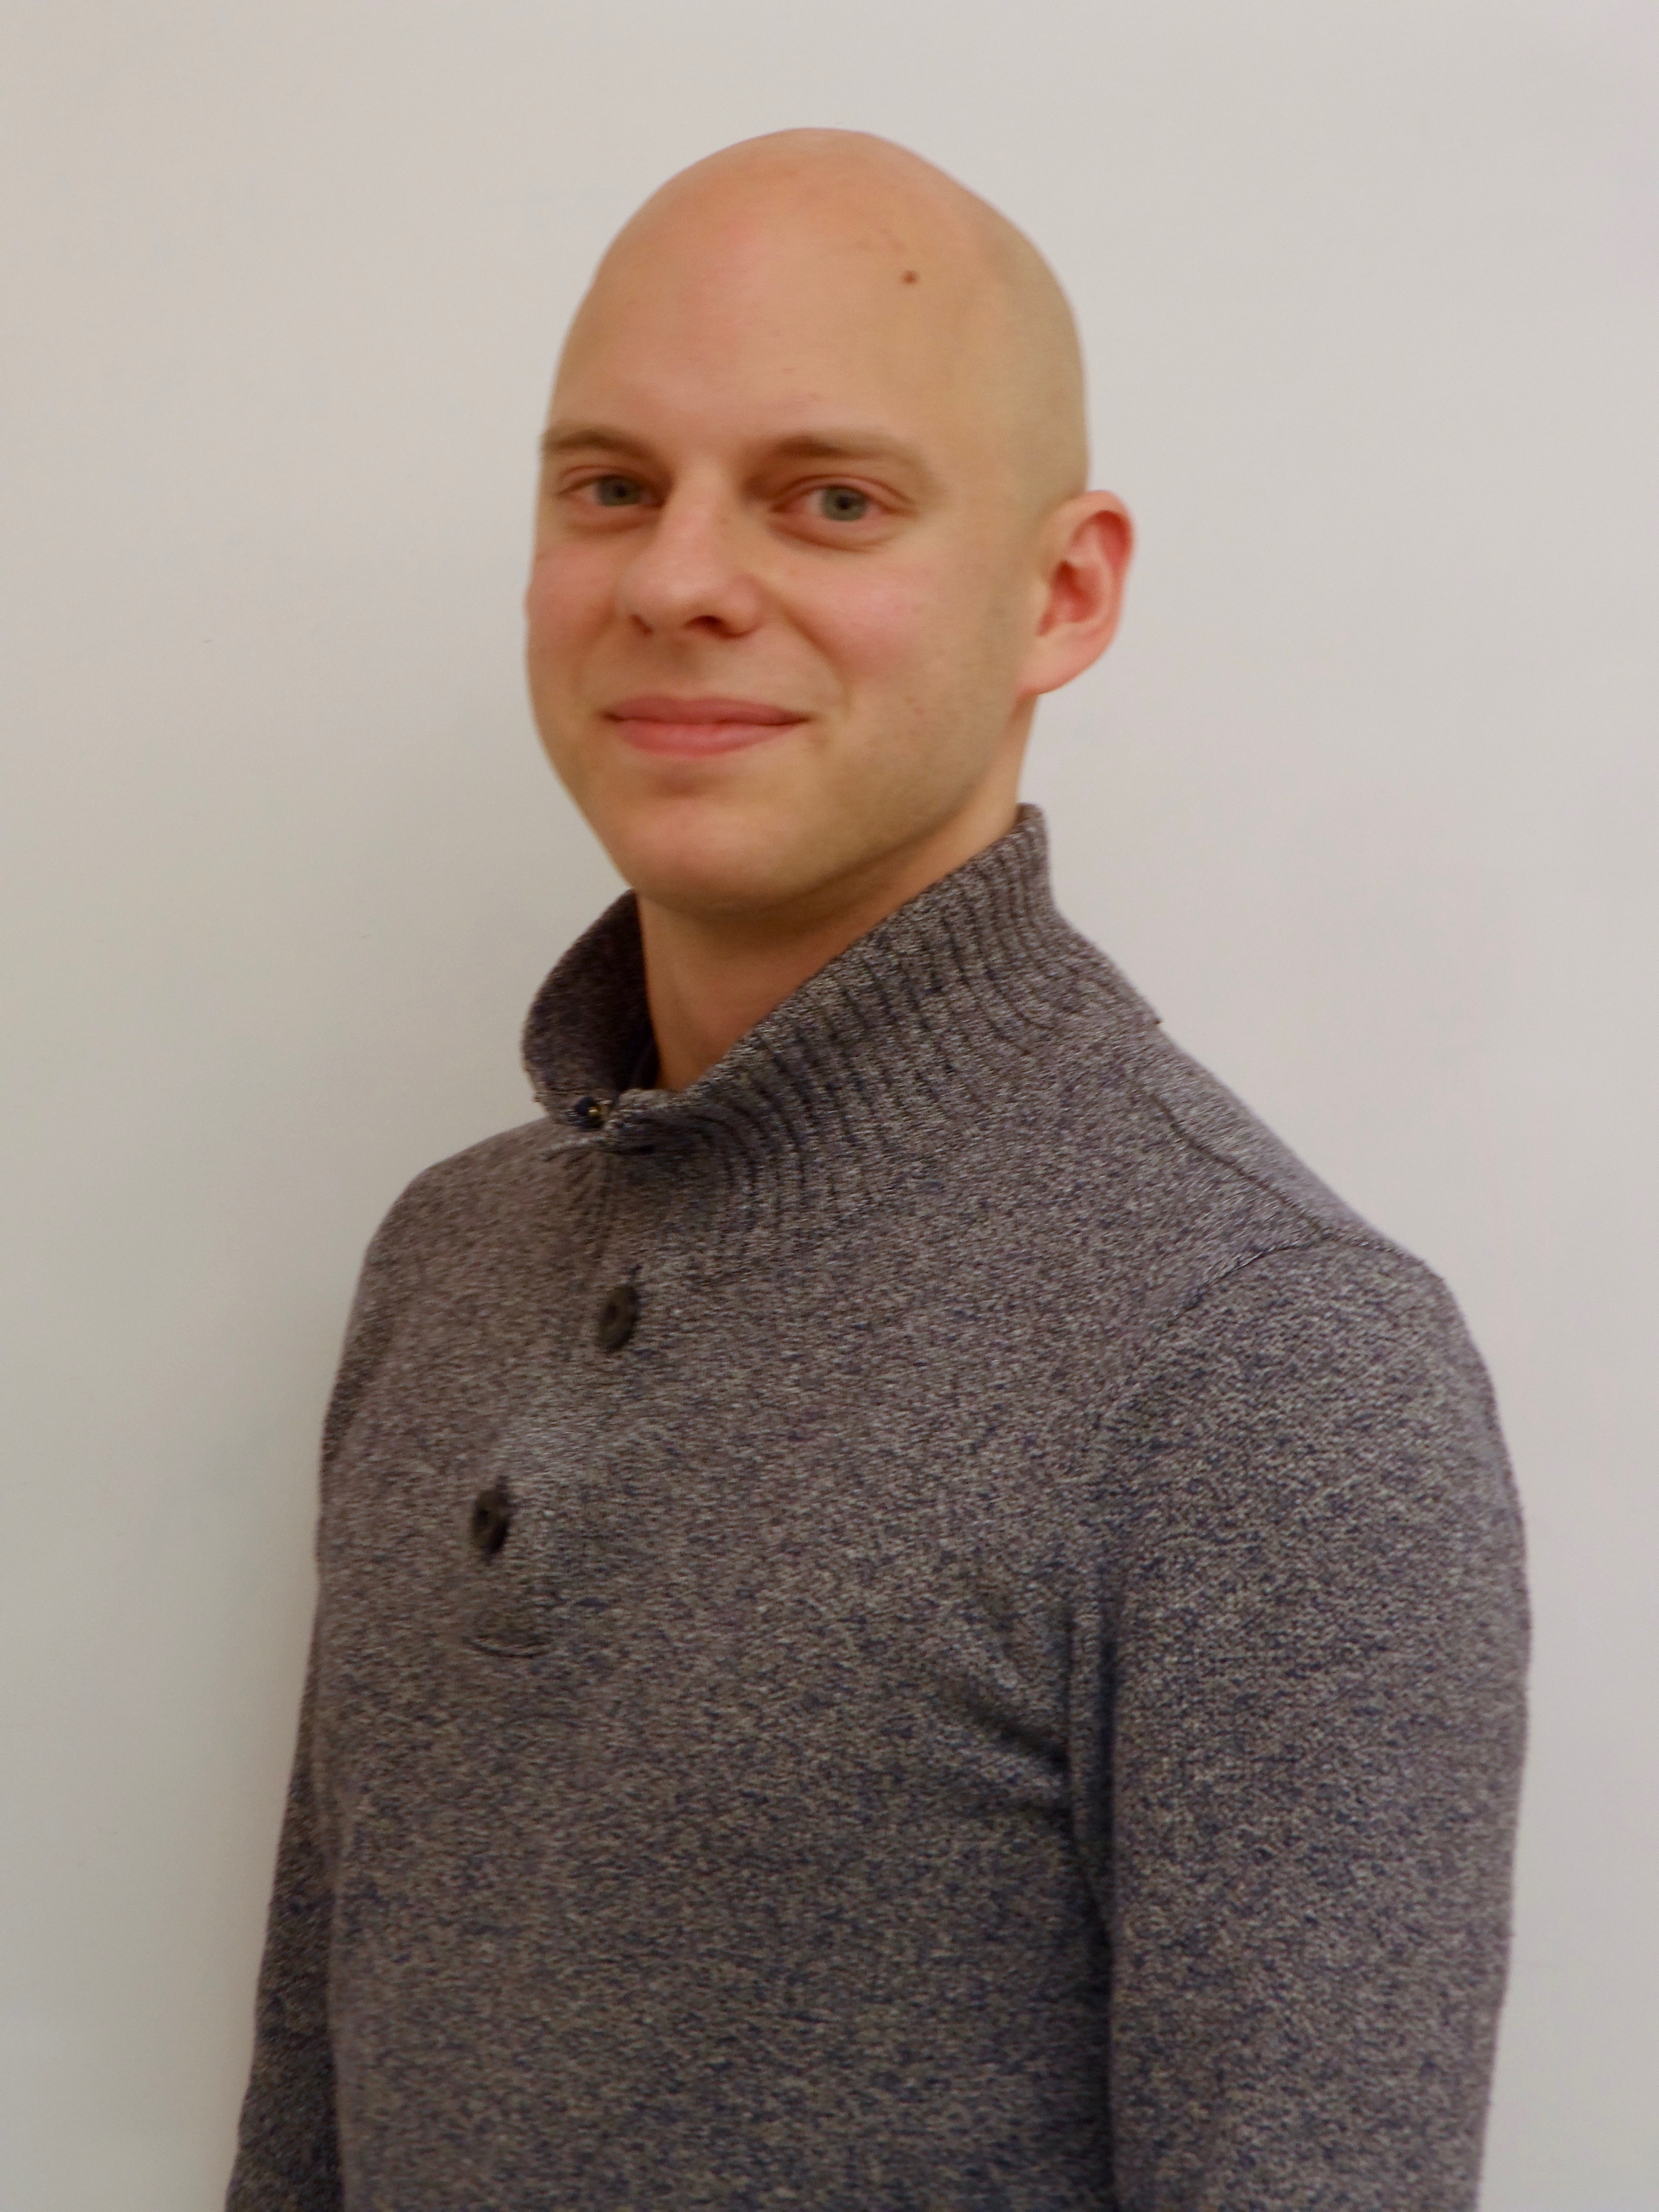
\includegraphics[width=35mm]{Figures/People/Jonathan}
\hspace{0.5em}\parbox[b]{0.6\textwidth}{\textbf{Jonathan Herdt}\\
Hasso Plattner Institute\\
Status: IT-Systems Engineering Master's degree student\\
Contact: jonathan.herdt@student.hpi.de\\
Skills: Design Thinking, Computer Science\\
}

I come from the Rhine-Neckar Metropolitan Region in Southern Germany and was born in Mannheim. Professionally, Heidelberg University was my first step to becoming a computer scientist because I completed a three year training there to become a computer science expert. I then earned my B.S. in Computer Science at Hochschule Mannheim (now also part of the SUGAR network). During my time as a student at Hochschule Mannheim, I spent two semesters abroad --- one in the US (College Park, MD) for an internship at Fraunhofer and one in Canada (St. John's, NL) for studying. I aim to take my education to another level by pursuing my M.S. in IT-Systems Engineering at Hasso Plattner Institute.

My main interest in my professional life is to create simple solutions. I enjoy getting to the heart of people's interactions with technology and what makes these interactions work or not work. This path has led me to discover Design Thinking for myself which goes a long way to ensuring that a user is at the heart of every creation and enhances my focus on simplicity with satisfying unfulfilled desires. ME310  was the next logical step in this direction for me and the outcome so far has shown me that this was the right decision.

%\begin{framed}
\vspace{2em}
\noindent 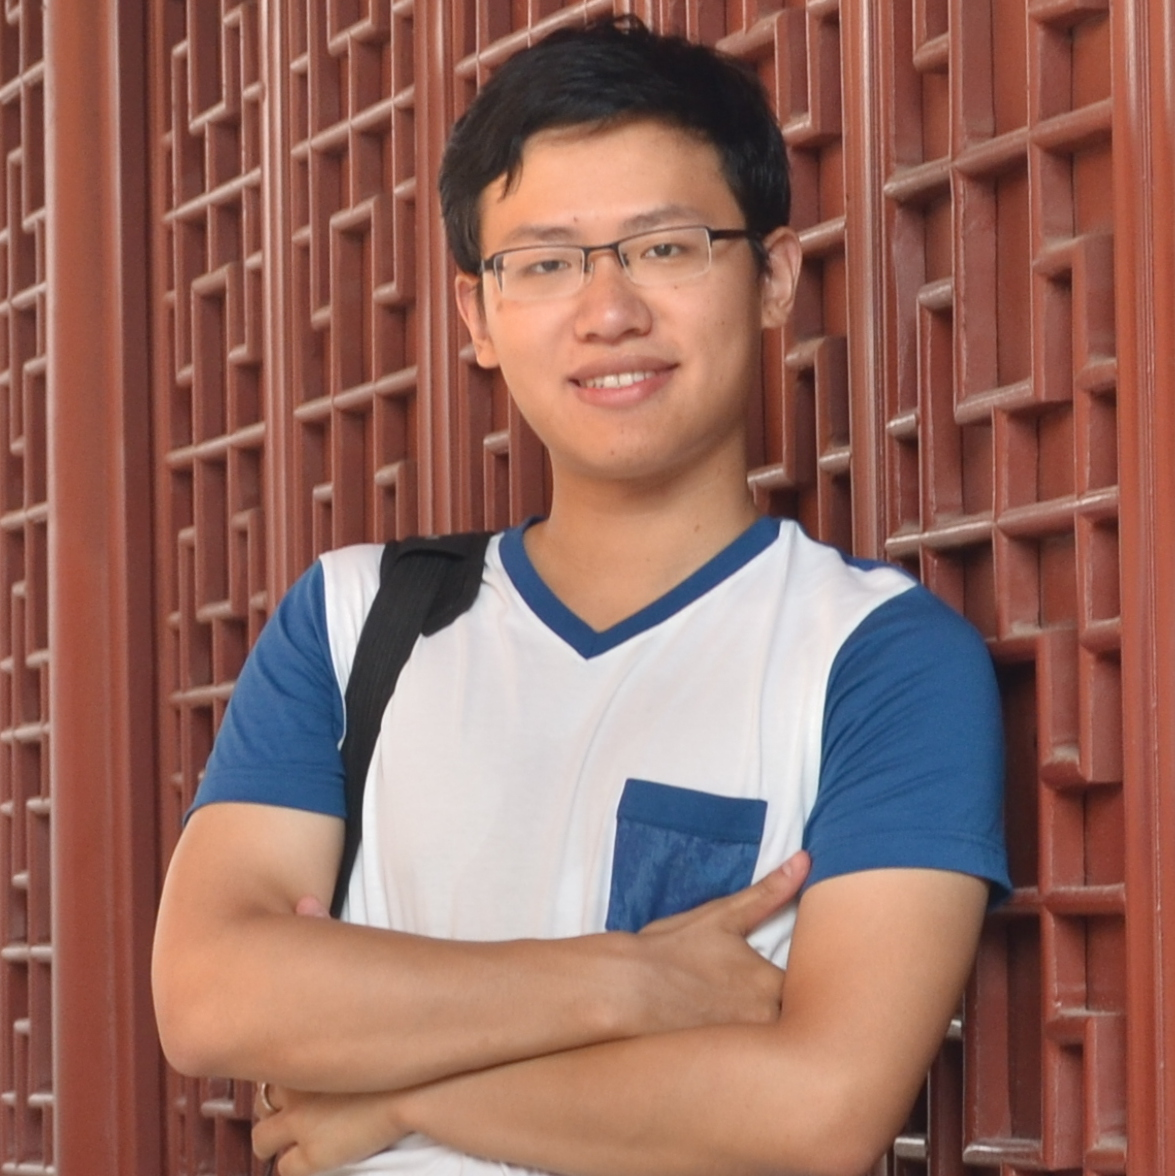
\includegraphics[width=35mm]{Figures/People/Zhipeng}
\hspace{0.5em}\parbox[b]{0.6\textwidth}{\textbf{Zhipeng Hu}\\
Stanford University\\
Status: M.E. first year Graduate Student\\
Contact: zhipengh@stanford.edu\\
Skills: Design, Mechatronics, Programming\\
}

I was born in Wuhan, a metropolis in the middle of China. I earned my Bachelor of Engineering degree in Mechanical Engineering at Tsinghua University, China.

I am interested in Mechatronics and Design. More specifically, I am fascinated by creative solution at systematic level and the interdisciplinary nature of Mechatronics area. As a Bachelor student, I have engaged in various design projects with topics such as embedded system, mechanical design, and virtual instrument. These experiences inspired me to further explore possibilities of smart product design, especially those within practical background. Moreover, during my undergraduate studies, I have focused on control theory and algorithms with application on precision motion control. It convinced me that smart products need a combination of hardware design and control software, which can be successfully integrated using design thinking.

%\end{framed}

%\begin{framed}
\vspace{2em}
\noindent 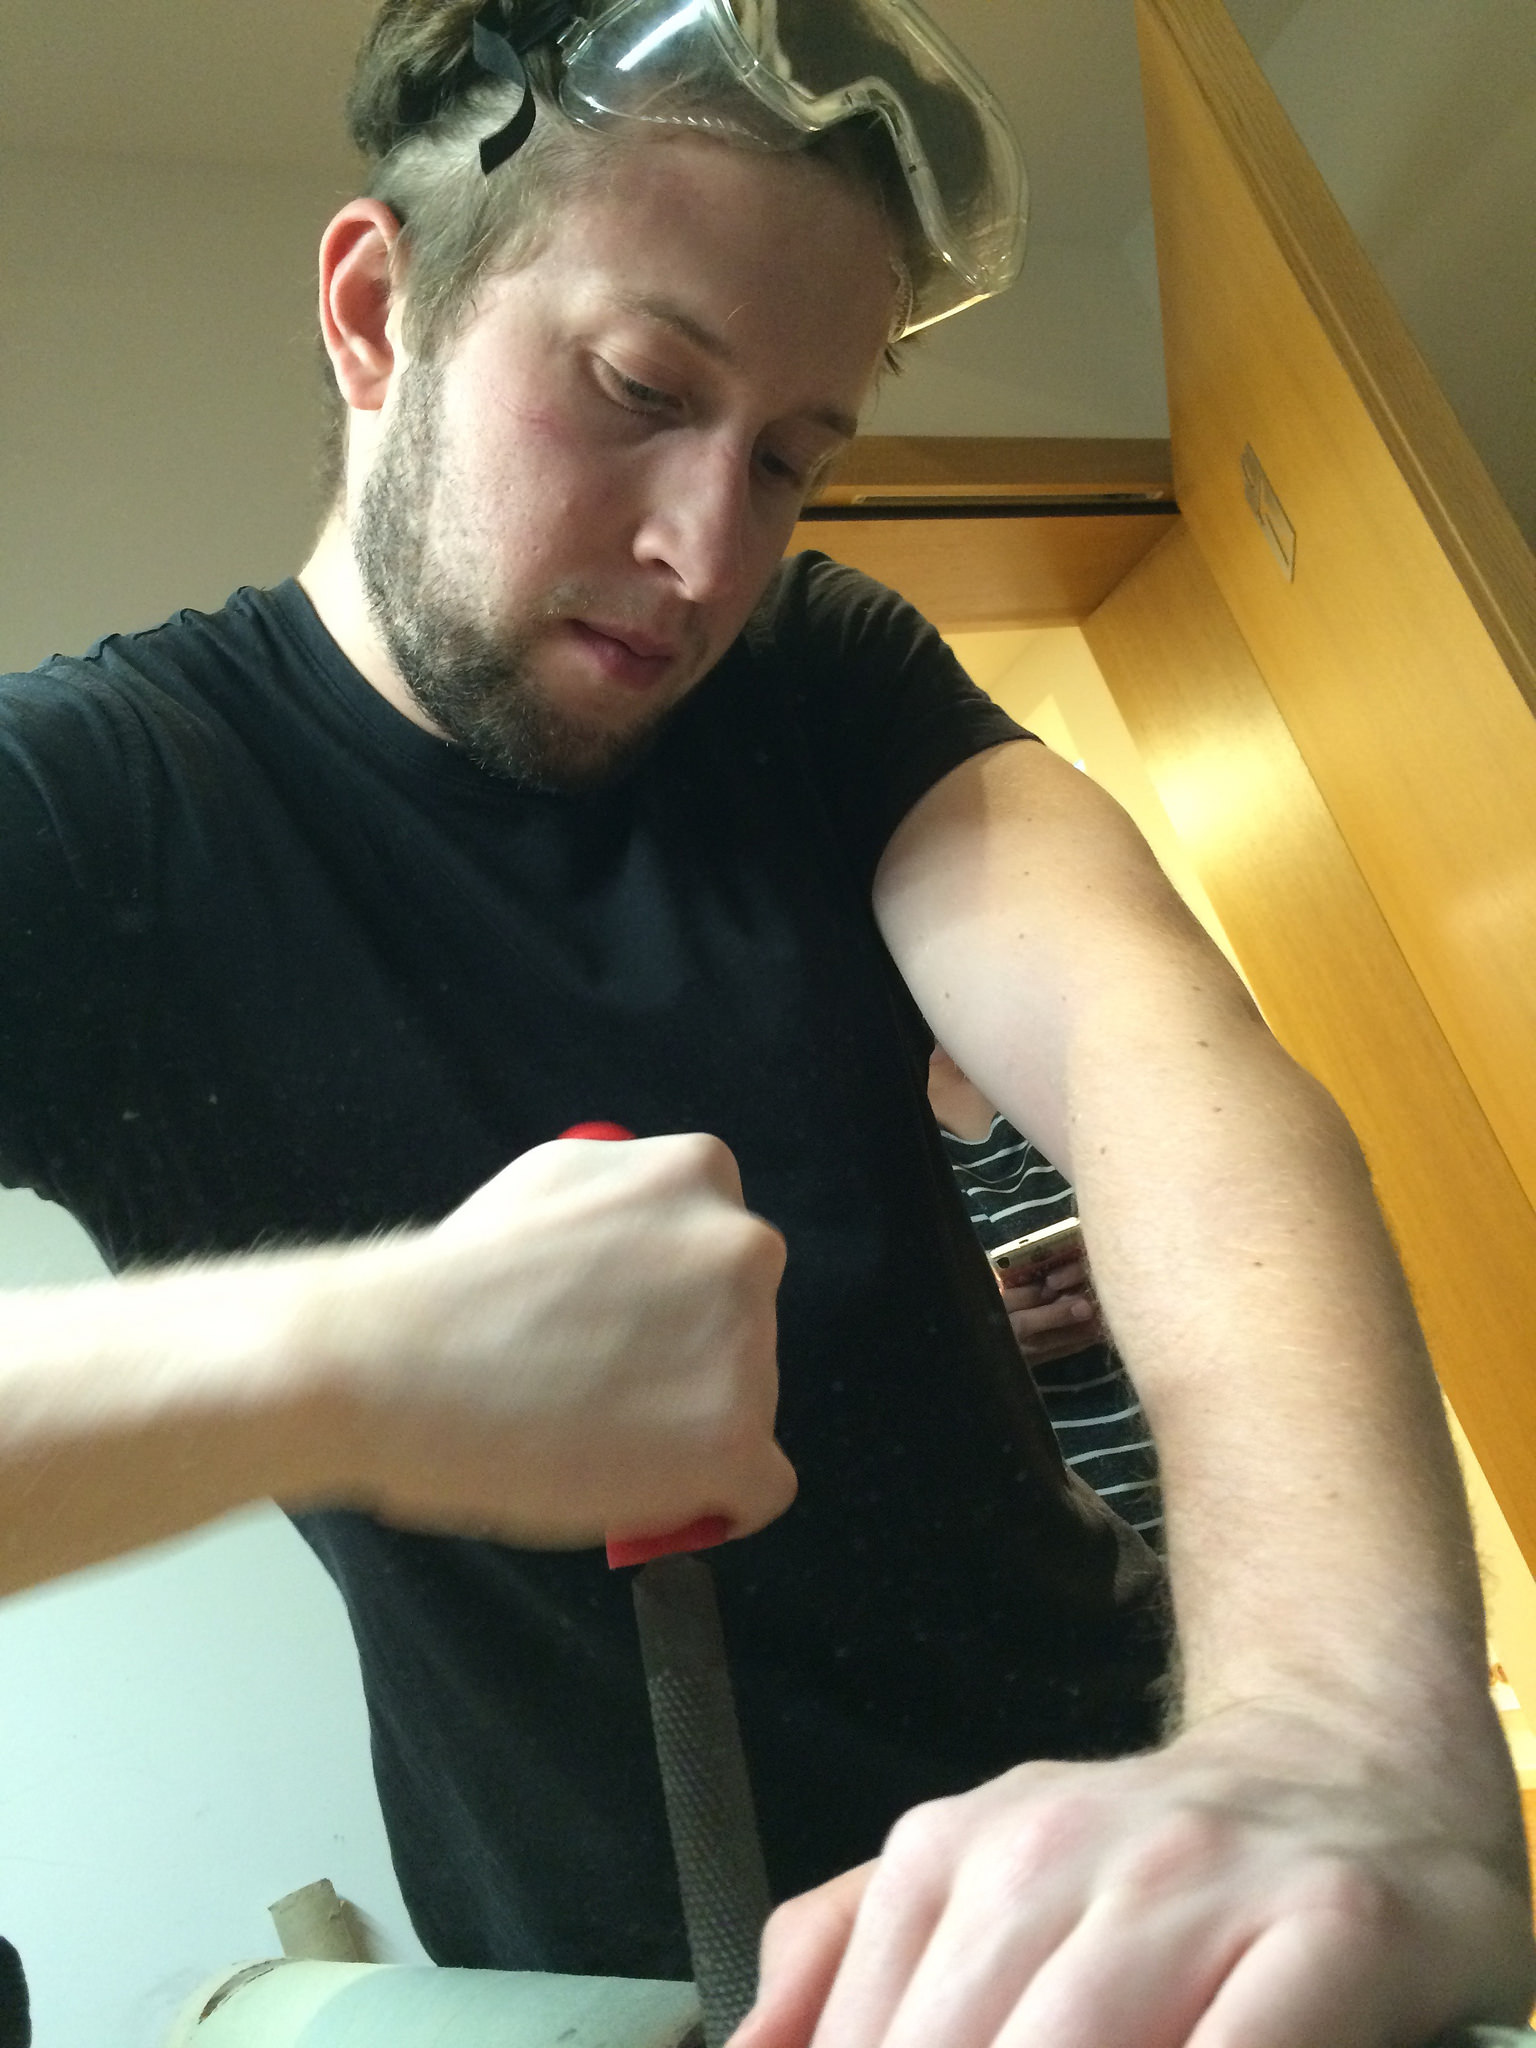
\includegraphics[width=35mm]{Figures/People/Jonas}
\hspace{0.5em}\parbox[b]{0.6\textwidth}{\textbf{Jonas Kemper}\\
Hasso Plattner Institute\\
Status: IT-Systems Engineering Master's degree student\\
Contact: jonas.kemper@student.hpi.de\\
Skills: Programming, Prototyping, Interaction design\\}

Born and raised in Germany near Cologne, I earned my Bachelor of Science degree from LMU Munich in Media Informatics and Human-Computer Interaction. Before starting to pursue a Master's degree at HPI, I programmed for and wrote my Bachelor's thesis about a cognitive architecture now based at MIT media lab. To continue this work, I was invited to attend two workshops held at the media lab (five weeks in 2014 and two weeks in 2015). I spent two quarters as a visiting computer science graduate student at UC San Diego where I also worked part-time at the design lab.

My interests span communication technology, concept development, and the business side of technology. These plus the multidisciplinary teams and the international community are why I am excited about the ME310 opportunity.
%\end{framed}

%\begin{framed}
\vspace{2em}
\noindent 
\includegraphics[width=35mm]{Figures/People/Johanna}
\hspace{0.5em}\parbox[b]{0.6\textwidth}{\textbf{Johanna Latt}\\
Hasso Plattner Institute\\
Status: IT-Systems Engineering Master's degree student\\
Contact: johanna.latt@student.hpi.de\\
Skills: Software Engineering, Mobile and VR Applications, Human Computer Interaction\\
}

I was born in Siegen, a city near Cologne, and grew up in a little village of 2,500 residents. I received my Bachelor of Science degree in Human-Computer Interaction from the University of Würzburg in Bavaria. Next to basics as psychology and methods of human-computer interaction, I also learned the basics of software engineering and worked in an IT company focusing on semantic web technologies during my time as undergraduate. In my bachelor thesis I worked on the topic of illusion of body ownership in virtual realities. Since I really enjoyed the computer science part of my studies I decided to apply at Hasso Plattner Institute for my master's degree, where I am currently in my 2nd semester.

I am fascinated by the human-centered design-thinking process of finding user needs and problems to develop meaningful and innovative applications and I love having the opportunity to walk through the full design cycle in the ME310 course, from the basic benchmarking and needfinding to the finished product, which unites my interests in psychology and computer science.
%\end{framed}

\vspace{2em}
\noindent 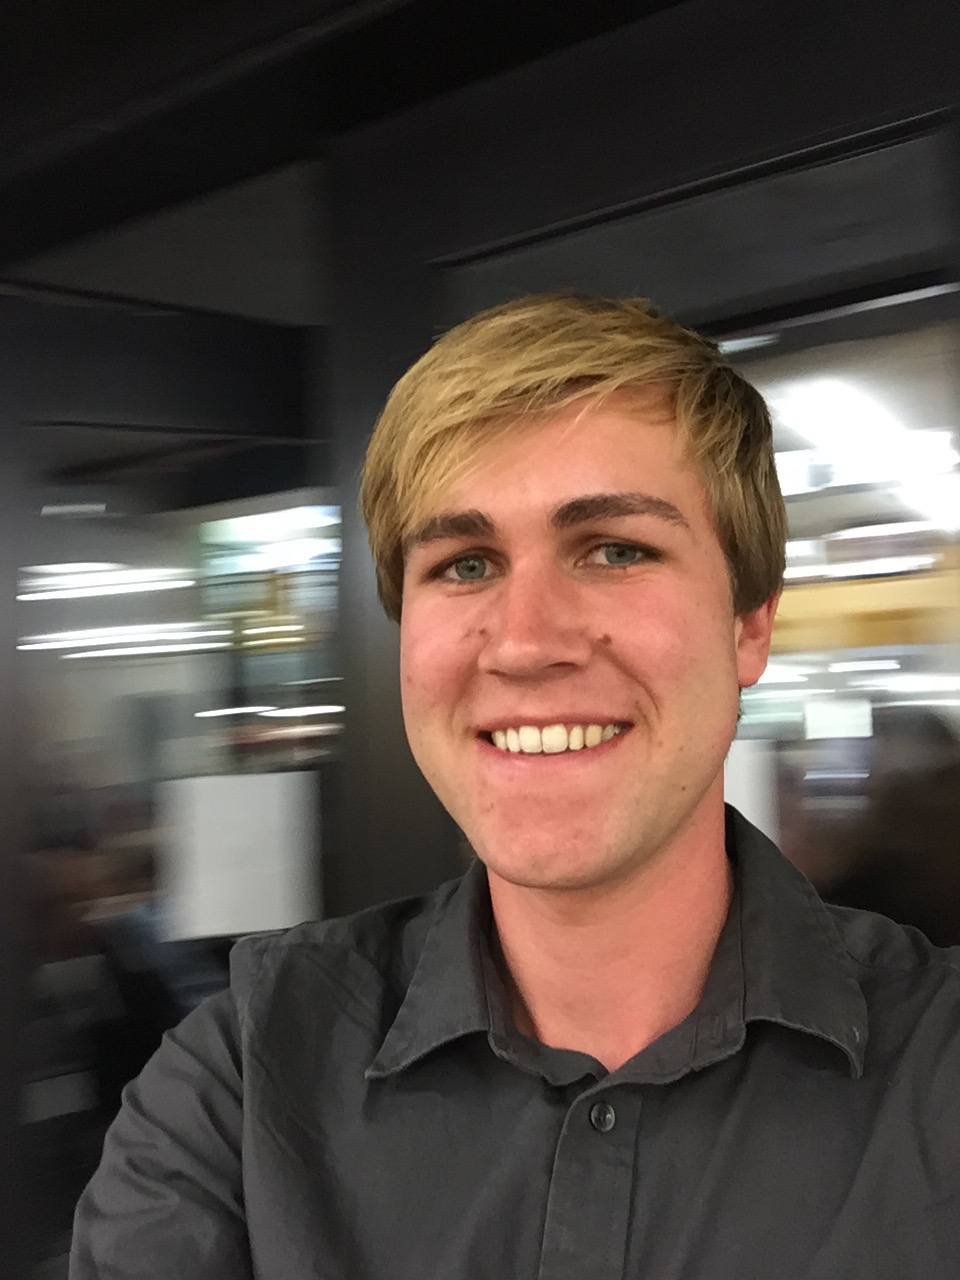
\includegraphics[width=35mm]{Figures/People/Dylan}
\hspace{0.5em}\parbox[b]{0.6\textwidth}{\textbf{Dylan Moore}\\
Stanford University\\
Status: First Year Mechanical Engineering Ph.D. Student\\
Contact: djmoore3@stanford.edu\\
Skills: Conceptual Design, User Experience, Systems Engineering, Research, Design Methodology, Graphic Design\\
}

I was born in Laguna Beach, CA and grew up in Orange County, CA. I received a B.S. in Engineering Physics and a B.A. in Music from UC Berkeley while an undergraduate and spent a summer studying abroad at the University of Cambridge in England. After Berkeley, I completed a Master’s at USC in Mechanical Engineering. I currently perform research on the design process in Professor Erin MacDonald's IRIS Design Lab. In the past, I have held several engineering internships and participated in research projects in the IMPACT laboratory at USC and Lawrence Berkeley National Lab.

I am incredibly curious about the world we live in, and I am interested in contributing to society in as many ways as I can.  I have a passionate drive for divergent creativity and problem solving, and I am excited about the opportunities and  experience ME310 offers. I bring a holistic and systems-level approach to the design team and look to integrate everyone's unique experience and perspectives into a unified vision.

%\end{framed}

\vspace{2em}
\noindent 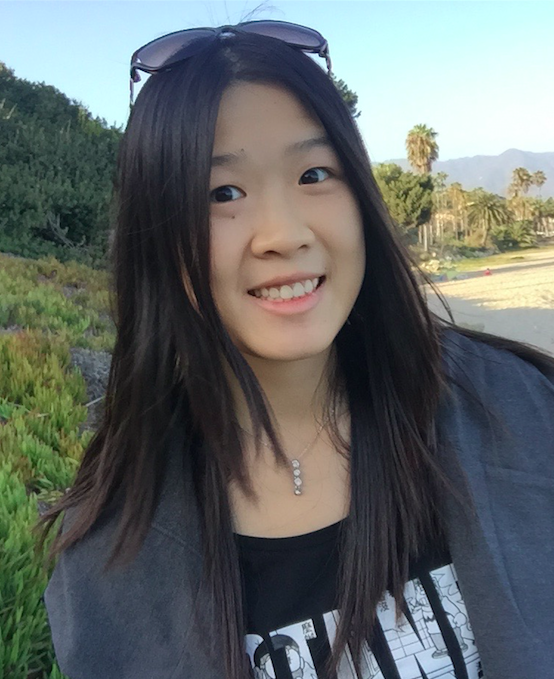
\includegraphics[width=35mm]{Figures/People/Maggie_Xu.png}
\hspace{0.5em}\parbox[b]{0.6\textwidth}{\textbf{Maggie Xu}\\
Stanford University\\
Status: First Year Mechanical Engineering Master Student\\
Contact: manqixu@stanford.edu\\
Skills: sketch, C++, violin\\
}

I grew up in China and received a B.S. degree in Mechanical Engineering from Tsinghua University in 2015. I'm interested in trying out new ideas and building stuff. I'm also curious about how the engineering design process could be improved through the interaction with other fields like physiology, humanity, or social science. My undergraduate major is precision instruments so most of my past design experiences are more focused on tiny devices like microchips for medical use. I had some mechatronics design experiences through class. I was an undergraduate visiting researcher at Stanford Mechanical Engineering Research Lab (MERL) in the summer of 2014, working on a droplet-based microfluidic chip for quantitative bacteria detection. In the winter of 2015, I was a research intern at the Centre for Advanced Photonics and Electronics (CAPE) at Cambridge University, designing the next generation of a star tracking system based on compressive sensing. Besides research, I've also completed a four-month marketing internship at Daimler AG, where I had a lot of fun and enjoyed the opportunity of understanding Mercedes-Benz cars from both an engineering side and a marketing side did help a lot in generating advertising ideas.
%\end{framed}

\clearpage

\subsection{Coaches}

\vspace{0.5em}
\noindent 
\includegraphics[width=35mm]{Figures/People/Scott_Henkelman.jpg}
\hspace{0.5em}\parbox[b]{0.6\textwidth}{\textbf{Scott Henkelman}\\
Scott Henkelman\\Stanford University\\
Status: Product Engineer, Private Technology Company\\
Contact: sjhenk@gmail.com\\
}
% \end{framed}

\vspace{2em}
\noindent 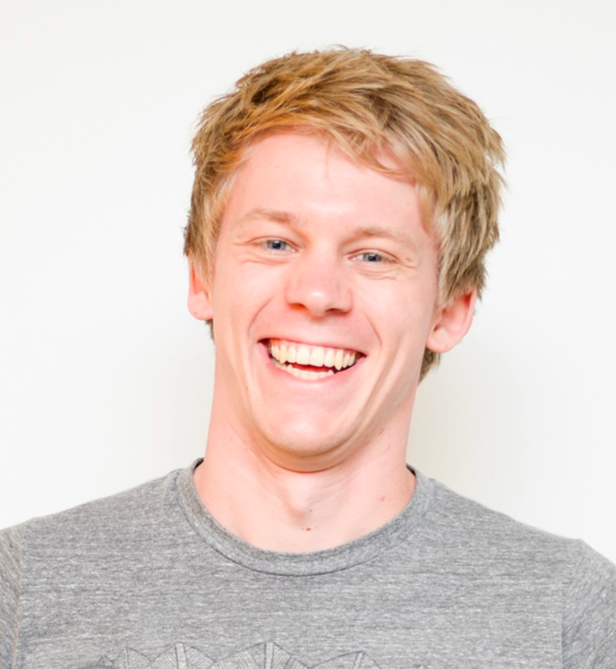
\includegraphics[width=35mm]{Figures/People/Max}
\hspace{0.5em}\parbox[b]{0.6\textwidth}{\textbf{Max Bothe}\\Hasso Plattner Institute\\
Status: IT-Systems Engineering Master's degree student\\
Contact: max.bothe@student.hpi.de\\
Skills: Software Engineering, iOS Development, Python\\
}

I was born in 1990 in a small town in Brandenburg, Germany. In 2009, I moved to Potsdam to start my Bachelor's studies at the Hasso Plattner Institute. Afterwards I joined SAP in Belfast, Northern Ireland, for software engineering internship for six months.
Currently I am again a computer science student at the Hasso Plattner Institute for getting my Master's degree. As part of my studies I am also working as a student assistant in the field of soccer analytics on databases.

I am interested in software engineering, iOS development, project management and creative design. I joined ME310 in 2014 developing a prototype of the must have features of the Audi ownership experience in 2025.

%\end{framed}

\section{What is ME310?}

\subsection{Design Thinking}

Design Thinking is the latest successor in a long-ranging history of research and development on design methods. More than half a century ago, in the mid-1960s, a need for a structured design process arose due to the rising complexities of developing technologies\footnote{Beckman, Sara L., and Michael Barry. "Innovation as a Learning Process: Embedding Design Thinking." (2007).}. Herbert Simon was the first to describe design as a "way of thinking"\footnote{Simon, Herbert Alexander. The sciences of the artificial. MIT press, 1969.}. Design Thinking grounds in the observation of how designers approach problems and how they develop new solutions\footnote{Cross, Nigel. Designerly ways of knowing. Springer London, 2006.}. 

According to David and Tom Kelley "Design Thinking is a way of finding human needs and creating new solutions using the tools and mindsets of design practitioners"\footnote{Kelley, Tom, and David Kelley. Creative confidence: Unleashing the creative potential within us all. Random House LLC, 2013.}. Design Thinkers combine empathy for the context of a problem, creativity in the generation of insights and solutions, and rationality in analysing and fitting various solutions to the problem context.
Although many tried to define what Design Thinking is\footnote{Razzouk, Rim, and Valerie Shute. "What is design thinking and why is it important?." Review of Educational Research (2012): 0034654312457429.}, there is still uncertainty whether to describe it as a methodology, a process or a mindset. For the sake of clarity we define Design Thinking as a methodology, attributed by three core elements: multidisciplinary teams, an iterative process and variable space (see figure~\ref{fig:d_process}).

\begin{figure}
  \centering
    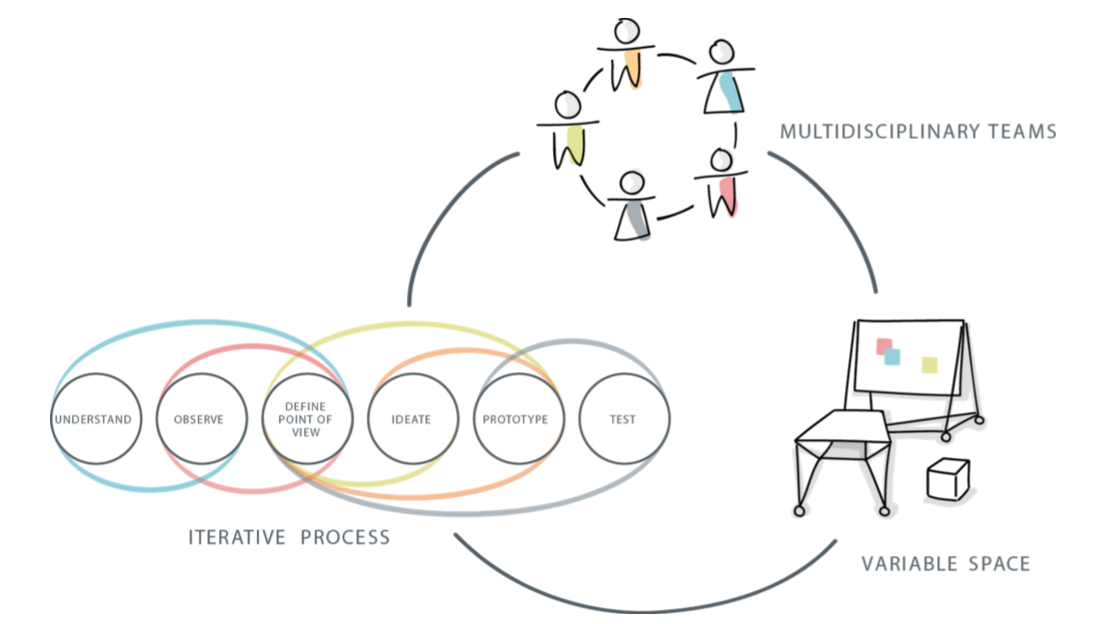
\includegraphics[width=1.0\textwidth]{Figures/ChapterContext/d_process}
  \caption[The Design-Thinking process]{© Prof. Ulrich Weinberg/HPI School of Design Thinking}
  \label{fig:d_process}
\end{figure}

\subsubsection{Process}

Kumar argues that "successful innovation can and should be planned and managed like any other organisational function"\footnote{Kumar, Vijay. 101 design methods: A structured approach for driving innovation in your organization. John Wiley \& Sons, 2012.}. And although his definition of the design process is different from Design Thinking, all approaches to design share great similarity in their attributes, e.g. being human-centered, non-linear, iterative and incremental. Brown explains the "continuum of innovation as a system of overlapping spaces called inspiration, ideation, and implementation"\footnote{Brown, Tim. Change by design. HarperCollins e-books, 2014.}, as opposed to a "predefined series of orderly steps". 

We use this iterative process to find out about people's hidden needs and match those with what is technologically feasible and what is viable in terms of business strategy. Key to the process is the strict separation between problem space and solution space. Within the first three steps we only focus on finding, selecting and understanding the right problem, which might be counter-intuitive as humans generally tend to think in solutions. The following steps, addressing the solution space, include the generation and selection of ideas, as well as their prototypical implementation and testing. This overall process is carried out in iterations, repeating it completely or partially as required.

\paragraph*{Mindset}

A key element of the process is the associated mindset that is an essential element of Design Thinking. Tim Brown defined guidelines for Design Thinking and some characteristics to look for in design thinkers that constitute the foundation to the Design Thinking mindset\footnote{Brown, Tim. "Design thinking." Harvard business review 86.6 (2008): 84.}. A more concrete definition is being provided by the d.school at Stanford University\footnote{The d.school bootcamp bootleg - \\\url{http://dschool.stanford.edu/wp-content/uploads/2011/03/BootcampBootleg2010v2SLIM.pdf}} and can be see in the figure~\ref{fig:d_mindset}.

\begin{figure}
  \centering
    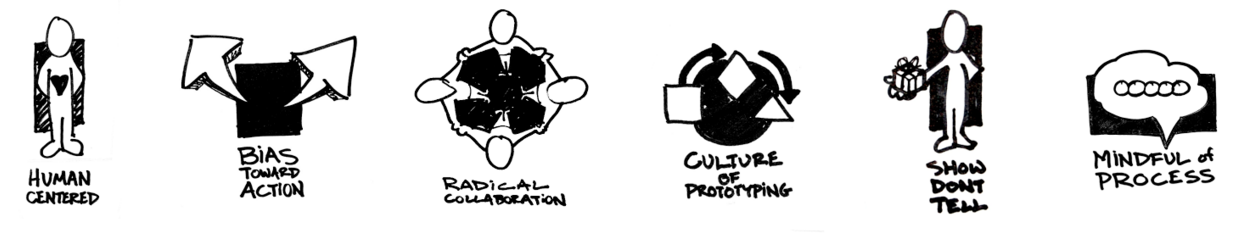
\includegraphics[width=0.9\textwidth]{Figures/ChapterContext/d_mindset}
  \caption[The Mindset of Design-Thinking]{© Hasso Plattner Institute of Design, Stanford University}
  \label{fig:d_mindset}
\end{figure}

\subsubsection{Space}

Part of the Design Thinking culture is an adaptable team working environment. Most furniture is on wheels and can be moved around once requirements change. Different spaces are available for collaborative working, building, communicating and presenting. Doorley et al. devoted a whole book on the design of creative spaces and view it as a necessity to foster collaboration.\footnote{Doorley, Scott, and Scott Witthoft. Make space: How to set the stage for creative collaboration. John Wiley \& Sons, 2011.}  Larry Leifer sees it as one of the three key factors that "influences the ideation and creative energy and output the most"\footnote{Leifer, Larry J, and Martin Steinert. "Dancing with ambiguity: Causality behavior, design thinking, and triple-loop-learning." Information, Knowledge, Systems Management 10.1 (2011): 151-173.}, the other two being absence of a fixed process and an overarching institutional practice of letting change happen. He states that it "lowers hierarchical boundaries, enhances ideation and creativity, fosters and accelerates prototyping and generally increases the rate of learning and change" (ibid.).

\subsubsection{Multidisciplinary Teams}

Brown et al. argue that "to achieve divergent thinking, it is important to have a diverse group of people involved in the process"\footnote{Brown, Tim, and Jocelyn Wyatt. "Design thinking for social innovation." (2010).}. A view that is also supported by Fay et al., who state that organisations more frequently rely on multidisciplinary teams as the increased complexity of tasks requires a wide breadth of knowledge, skills and abilities\footnote{Fay, Doris et al. "Getting the most out of multidisciplinary teams: A multi-sample study of team innovation in health care." Journal of Occupational and Organizational Psychology 79.4 (2006): 553-567.}. This view holds that diversity will lead to an increase in the variety of perspectives and approaches and hence lead to greater creativity and quality of team performance\footnote{Mannix, Elizabeth, and Margaret A Neale. "What differences make a difference? The promise and reality of diverse teams in organizations." Psychological science in the public interest 6.2 (2005): 31-55.}.

\subsection{ME310/SUGAR}

The nine-month graduate level engineering course ME310 has been created over forty years ago at Stanford University and aims to provide engineering students with real-life engineering challenges. The name is derived from the course labelling scheme at Stanford and is short for Mechanical Engineering 310.

Over time, the course evolved to reflect the characteristics of today’s business environment, such as remote, intercultural collaboration, industry alliances, and services orientation.  It has grown beyond the hedges of Stanford University and is currently taught at over twenty universities spread across five continents . This global innovation network is known by the name SUGAR\footnote{Sugar Network - http://sugar-network.org }. The course is now focused on teaching students the innovation methods and processes required for designers, engineers and project managers of the future\footnote{Carleton, T, and L Leifer. "Stanford’s ME310 course as an evolution of engineering design." Proceedings of the 19th CIRP Design Conference–Competitive Design 31 Mar. 2009.}. Therefore student teams work on innovation challenges posed by corporate partners over a duration of nine months. Throughout the projects, students traverse an intense and iterative process of discovering problems and designing and testing various solutions in order to develop a functioning proof-of-concept prototype. The different phases involve need-finding, ideation, rapid prototyping and testing. The course uses Design Thinking to facilitate the human-centred design process. An approach has been recognised as essential for the social acceptance of a solution.

For the duration of each project, each team within the network pairs with another team from a foreign university to jointly solve the proposed design challenge. These partnerships add diversity to the project teams and give students the opportunity to experience true international collaboration, which is an essential skill required in this highly globalised world.

Company involvement provides the reality that is crucial for teams to improve their innovation abilities. In the end, teams deliver functioning prototypes along with in-depth documentation that not only captures the essence of the designs, but also the rationale behind their ideas.

\subsubsection{Project \& Team Setup}

Project teams within ME310 and SUGAR Projects usually consist of two sub-teams from different universities with 3-4 students respectively. The global team comprises participants from various disciplines. This form of interdisciplinary teamwork involves participants working jointly with the objective to find a coherent and holistic end result by analysing, synthesising and harmonising different disciplines. 
The work of each sub-team is facilitated by a dedicated teaching team and project coaches. Often external partner and alumni are invited to coach specific topics, in order to improve communication or to learn how to deal with cultural differences. 

\subsubsection{Process}

\begin{figure}
  \centering
   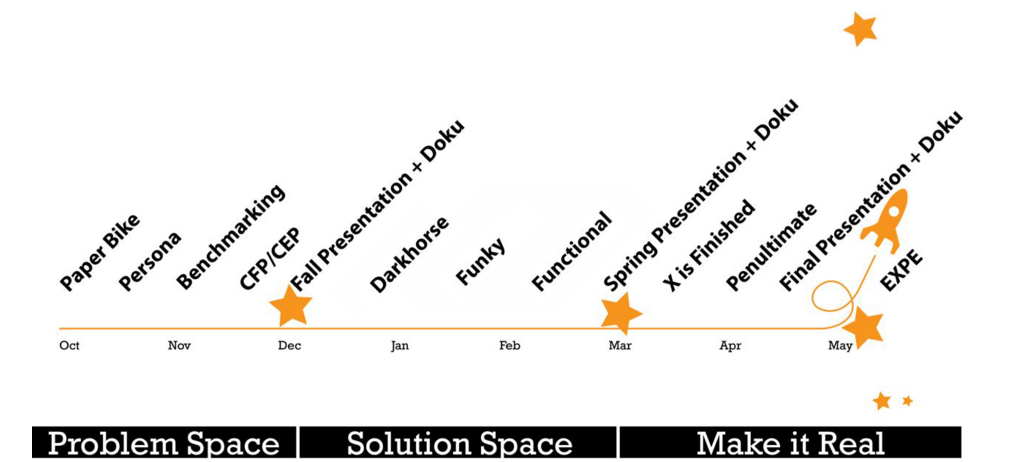
\includegraphics[width=0.9\textwidth]{Figures/ChapterContext/me310_timeline}
   \caption{The ME310-timeline}
  \label{fig:me310_timeline}
\end{figure}

ME310 and SUGAR projects provide a high-level process that rests upon a set of prototypes that define different stages of the design (figure~\ref{fig:me310_timeline}). The course starts with benchmarking and need-finding and continues with the development of exploratory prototypes to foster understanding. The first quarter ending with the autumn presentation and documentation hence mostly considers problem understanding and is defined as the Problem Space. The next quarter focuses on the exploration of the Solution Space, where first parts of the final concept are developed and tested individually. The last quarter, labeled Make it real, serves to integrate the discovered solutions into a complex system prototype. 